\chapter{Variables and functions}
% last edited 2008-11-22
 
% 6. 
\section{Variables and constants} 

A {\it variable} is a quantity to which an unlimited number of values 
can be assigned. Variables are denoted by the later letters of 
the alphabet. Thus, in the equation of a straight line,

\[
    \frac{x}{a} + \frac{y}{b} = 1
\]
$x$ and $y$ may be considered as the variable coordinates of a 
point moving along the line.
\index{variable}
A quantity whose value remains unchanged is called a {\it constant}.
\index{constant}

Numerical or absolute constants retain the same values in all problems, 
as $2$, $5$, $\sqrt{7}$, $\pi$, etc.

{\it Arbitrary constants, or parameters}, are constants to which any 
one of an unlimited set of numerical values may be assigned, 
and they are supposed to have these assigned values throughout 
the investigation. They are usually denoted by the earlier 
letters of the alphabet. Thus, for every pair of values arbitrarily 
assigned to $a$ and $b$, the equation

\[
    \frac{x}{a} + \frac{y}{b} = 1
\]
represents some particular straight line.
\index{parameters}


% 7. 
\section{Interval of a variable} 

Very often we confine ourselves 
to a portion only of the number system. For example, we may 
restrict our variable so that it shall take on only such values 
as lie between $a$ and $b$, where $a$ and $b$ may be included, or 
either or both excluded. We shall employ the symbol 
$\left \lbrack a,\ b \right \rbrack$, $a$ being less than $b$, 
to represent the numbers $a,\ b$, and all the numbers between 
them, unless otherwise stated. This symbol 
$\left \lbrack a,\ b \right \rbrack$ is read the interval from 
$a$ to $b$.


% 8. 
\section{Continuous variation} 

A variable $x$ is said to vary continuously 
through an interval $\left \lbrack a,\ b \right \rbrack$, when 
$x$ starts with the value $a$ and increases until it takes on 
the value $b$ in such a manner as to assume the value of every 
number between $a$ and $b$ in the order of their magnitudes. 
This may be illustrated geometrically as follows:


\begin{figure}[h]
\begin{minipage}{\textwidth}
\begin{center}
%\vspace{1.0 cm}
%
\includegraphics[height=1cm,width=8cm]{interval_AB.eps}
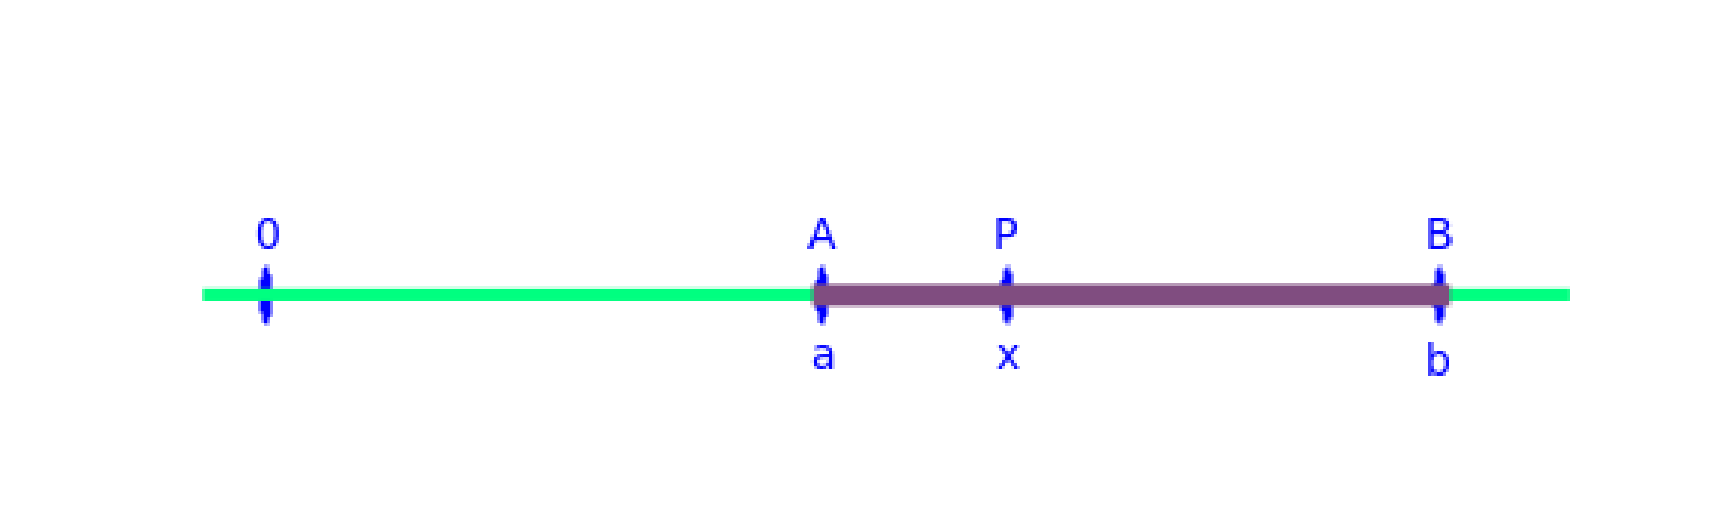
\includegraphics[height=2.5cm,width=8cm]{line-segment.eps}
\end{center}
\end{minipage}
\caption{Interval from $A$ to $B$.}
\label{fig:AB}
\end{figure}
%sage: f = lambda x: 0
%sage: G1 = plot(f, -5, 6, thickness=3, rgbcolor=(0.0,1,0.5))
%sage: G2 = plot(f, 0, 5, thickness=5, rgbcolor=(0.5,0.3,0.5))
%sage: t1 = text('A', (0.0, 0.1))
%sage: t2 = text('B', (5.0, 0.1))
%sage: t3 = text('0', (-4.5, 0.1))
%sage: p1 = disk((0.0, 0.0), 0.05, (0, 2*pi))
%sage: p2 = disk((5.0, 0.0), 0.05, (0, 2*pi))
%sage: p3 = disk((-4.5, 0.0), 0.05, (0, 2*pi))
%sage: show(G1+G2+t1+t2+t3+p1+p2+p3,axes=False)

\noindent
The origin being at $O$, layoff on the straight line the points 
$A$ and $B$ corresponding to the numbers $a$ and $b$. Also 
let the point $P$ correspond to a particular value of the variable $x$. 
Evidently the interval $\left \lbrack a,\ b \right \rbrack$ is 
represented by the segment $AB$. Now as $x$ varies continuously 
from $a$ to $b$ inclusive, i.e. through the interval 
$\left \lbrack a,\ b \right \rbrack$, the point $P$ 
generates the segment $AB$.


% 9. 
\section{Functions} 

When two variables are so related that the 
value of the first variable depends on the value of the second 
variable, then the first variable is said to be a {\it function} of 
the second variable.
\index{function}

Nearly all scientific problems deal with quantities and relations 
of this sort, and in the experiences of everyday life we are 
continually meeting conditions illustrating the dependence of 
one quantity on another. For instance, the weight a man is able 
to lift depends on his strength, other things being equal. 
Similarly, the distance a boy can run may be considered as 
depending on the time. Or, we may say that the area of a square 
is a function of the length of a side, and the volume of a 
sphere is a function of its diameter.


\vskip .1in

\begin{Verbatim}[fontsize=\tiny,fontfamily=courier,fontshape=tt,frame=single,label=\sage]

sage: I1 = interval(1,3)
sage: I2 = interval(2,6)
sage: I3 = interval(min(I2),max(I1)) # the intersection
sage: P1 = plot(0, xmin=min(I1), xmax = max(I1), thickness=10, rgbcolor=(1,0,0),linestyle="--")
sage: P2 = plot(0, xmin=min(I2), xmax = max(I2), thickness=10, rgbcolor=(0,1,0),linestyle=":")
sage: P3 = plot(0, xmin=min(I3), xmax = max(I3), thickness=10, rgbcolor=(1,1,0))
sage: show(P1+P2+P3)

\end{Verbatim}

\begin{figure}[h]
\begin{minipage}{\textwidth}
\begin{center}
%\vspace{1.0 cm}
%
\includegraphics[height=1cm,width=8cm]{interval_AB.eps}
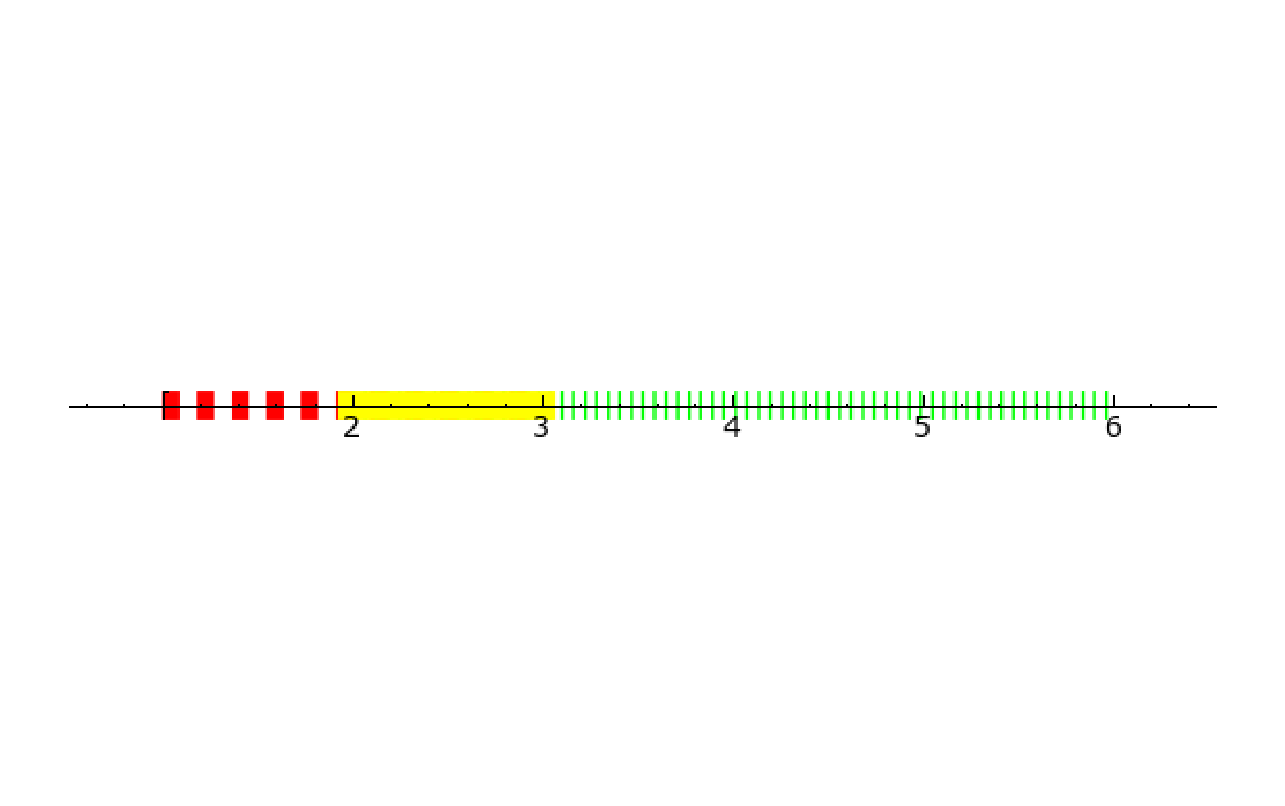
\includegraphics[height=2.5cm,width=8cm]{intervals-ch2a.eps}
\end{center}
\end{minipage}
\caption{Interval $[1,3]$ is dashed, $[2,5]$ is dotted, $[1,3]\cal [2,5]=[2,3]$ is solid.}
\label{fig:interval-cha2a}
\end{figure}


% 10
\section{Independent and dependent variables} 

The second variable, 
to which values may be assigned at pleasure within limits 
depending on the particular problem, is called the {\it independent 
variable}, or {\it argument}; and the first variable, whose value is 
determined as soon as the value of the independent variable is 
fixed, is called the {\it dependent variable}, or {\it function}.
\index{argument}
\index{independent variable}
\index{dependent variable}
\index{function}

Frequently, when we are considering two related variables, it is 
in our power to fix upon whichever we please as the independent 
variable; but having once made the choice, no change of 
independent variable is allowed without certain precautions and 
transformations.

One quantity (the dependent variable) may be a function of two 
or more other quantities (the independent variables, or arguments). 
For example, the cost of cloth is a function of both the 
quality and quantity; the area of a triangle is a function of 
the base and altitude; the volume of a rectangular parallelepiped 
is a function of its three dimensions.

In the \sage example below, $t$ is the independent variable and 
$f$ is the dependent variable. Though this example uses differentiation
(\sage's {\tt f.diff} notation), you don't need to understand
how to differentiate to appreciate the syntax \sage uses 
to express the command.

\vskip .1in

\begin{Verbatim}[fontsize=\scriptsize,fontfamily=courier,fontshape=tt,frame=single,label=\sage]
sage: t = var('t')
sage: f = function('f', t)
sage: f(t).diff(t)
diff(f(t), t, 1)
sage: (2*f(t)+3).diff(t)
2*diff(f(t), t, 1)
sage: (f(t)^2).diff(t)
2*f(t)*diff(f(t), t, 1)
sage: f = cos
sage: f(pi/2)
0
sage: f(t).diff(t)
-sin(t)

\end{Verbatim}


% 11
\section{Notation of functions}

The symbol $f(x)$ is used to denote a function of $x$, and is 
read ``$f$ of $x$''. In order to distinguish between different 
functions, the prefixed letter is changed, as $F(x)$,\ $\phi(x)$,\ $f'(x)$, 
etc.

During any investigation the same functional symbol always 
indicates the same law of dependence of the function upon the variable. 
In the simpler cases this law takes the form of a series of 
analytical operations upon that variable. Hence, in such a case, 
the same functional symbol will indicate the same operations 
or series of operations, even though applied to different 
quantities. Thus, if

\[
f(x) = x^2 - 9x + 14,
\]
then 	
\[
f(y) 	= y^2 - 9y + 14.
\]
Also 	
\[f(a) 	= a^2 - 9a + 14,
\]
\[
f(b + 1) = (b + 1)^2 - 9(b + 1) + 14 = b^2 - 7b + 6,
\]
\[
f(0) 	= 0^2 - 9 \cdot 0 + 14 = 14,
\]
\[
f(-1) 	= (-1)^2 -9(-1) + 14 = 24,
\]
\[
f(3) 	= 3^2 -9 \cdot 3 + 14 = -4,
\]
\[
f(7) 	= 7^2 -9 \cdot 7 + 14 = 0,
\]
etc.
Similarly, $\phi(x,\ y)$ denotes a function of $x$ and $y$, 
and is read ``$\phi$ of $x$ and $y$''.
If 	
\[
\phi(x,\ y) 	= \sin(x + y),
\]
then 	
\[
\phi(a,\ b) 	= \sin(a + b),
\]
and 	
\[
\phi \left ( \frac{\pi}{2}, 0 \right )	= \sin \frac{\pi}{2} = 1.
\]
Again, if 	
\[
F( x,\ y,\ z ) 	= 2x + 3y - 12z,
\]
then 	
\[
F(m,\ -m,\ m) 	= 2m - 3m - 12m = - 13m.
\]
and 	
\[
F(3,\ 2,\ 1) 	= 2 \cdot 3 + 3 \cdot 2 - 12 \cdot 1 = 0.
\]
Evidently this system of notation may be extended indefinitely.

You can define a function in \sage in several ways:

\vskip .1in

\begin{Verbatim}[fontsize=\scriptsize,fontfamily=courier,fontshape=tt,frame=single,label=\sage]

sage: x,y = var("x,y")
sage: f = log(sqrt(x))
sage: f(4)
log(4)/2
sage: f(4).simplify_log()
log(2)
sage: f = lambda x: (x^2+1)/2
sage: f(x)
(x^2 + 1)/2
sage: f(1)
1
sage: f = lambda x,y: x^2+y^2
sage: f(3,4)
25
sage: R.<x> = PolynomialRing(CC,"x")
sage: f = x^2+2
sage: f.roots()
[(1.41421356237309*I, 1), (2.77555756156289e-17 - 1.41421356237309*I, 1)]

\end{Verbatim}

\vskip .1in
\noindent


% 12
\section{Values of the independent variable for which a function is defined}

Consider the functions
\[
    x^2 - 2x + 5,\ \sin x,\ \arctan x
\]
of the independent variable $x$. Denoting the dependent variable 
in each case by $y$, we may write

\[
    y = x^2 - 2 x + 5,\ y = \sin x,\ y = \arctan x.
\]
In each case $y$ (the value of the function) is known, or, 
as we say, defined, for all values of $x$. This is not by any 
means true of all functions, as the following examples 
illustrating the more common exceptions will show.

\begin{equation}
%(1) 
y = \frac{a}{x - b}
\label{eqn:1}
\end{equation}
Here the value of $y$ (i.e. the function) is defined for all values 
of $x$ except $x = b$. When $x = b$ the divisor becomes zero and 
the value of $y$ cannot be computed from (\ref{eqn:1}).
Any value might be assigned to the function for this value of the argument.

\begin{equation}
%(2) 
y = \sqrt{x}.
\label{eqn:2}
\end{equation}
In this case the function is defined only for positive values of $x$. 
Negative values of $x$ give imaginary values for $y$, and these must 
be excluded here, where we are confining ourselves to real numbers only.

\begin{equation}
%(3) 
y = \log_a{x}. \qquad a > 0
\label{eqn:3}
\end{equation}
Here $y$ is defined only for positive values of $x$. 
For negative values of $x$ this function does not exist (see 
\ref{sec:19}).

\begin{equation}
%(4) 
y = \arcsin x,\ y = \arccos x.
\label{eqn:4}
\end{equation}
Since sines, and cosines cannot become greater than $+1$ nor 
less than $-1$, it follows that the above functions are 
defined for all values of $x$ ranging from $-1$ to $+1$ 
inclusive, but for no other values.

\vskip .1in

\begin{Verbatim}[fontsize=\scriptsize,fontfamily=courier,fontshape=tt,frame=single,label=\sage]

sage: t = var("t'')
sage: f = function('f', t)
sage: g = function('g', t)
sage: f = sin
sage: g = asin
sage: f(g(t))
t
sage: g(f(t))
t
sage: g(f(0.2))
0.200000000000000

\end{Verbatim}

%\vskip .3in
%\begin{center}
%{\bf Exercises}
%\end{center}
%\vskip .2in

\section{Exercises}


\begin{enumerate}
\item
% 1.
Given $f(x) = x^3 - 10x^2 + 31x - 30$; show that

\[
f(0) 	= -30,\ \ \ \ f(y) = y^3 - 10y^2 + 31y - 30,
\]
\[
f(2) = 0,\ \ \ \  f(a) 	= a^3 - 10a^2 + 31a - 30,
\]
\[
 f(3) =	f(5),\ \ \ \ 
f(yz) 	= y^3z^3 - 10y^2z^2 + 31yz - 30,
\]
\[
   f(1) > f( − 3),\ \ \ \ 
f(x − 2) 	= x^3 - 16x^2 + 83x - 140,
\]
\[
  f( - 1) 	= 6f(6). 
\]

\item
%2. 
If $f(x) = x^3 - 3x + 2$, find $f(0)$,\ $f(1)$,\ $f(-1)$,\ 
$f \left ( -\frac{1}{2} \right )$,\ 
$f \left ( \frac{4}{3} \right )$.

\item
%3. 
If $f(x) = x^3 - 10x^2 + 31x - 30$, and 
$\phi (x) = x^4 − 55x^2 − 210x − 216$, show that

$f(2) = \phi ( - 2)$,
$f(3) = \phi( - 3),f(5) = \phi( - 4)$,
$f(0) + \phi (0) + 246 = 0$.

\item
%4. 
If $F(x) = 2x$, find $F(0)$,\ $F(-3)$,\ 
$F \left ( \frac{1}{3} \right )$,\ $F(-1)$.

\item
%5. 
Given $F(x) 
= x(x - 1)(x + 6) \left ( x - \frac{1}{2} \right ) 
\left (x + \frac{5}{4} \right )$, show that
$F(0) = F(1) = F(-6) = F \left (\frac{1}{2} \right ) 
= F \left ( -\frac{5}{4} \right ) = 0$. 

\item
%6
If $f(m_1) = \frac{m_1 - 1}{m_1 + 1}$, show that
$\frac{f(m_1) - f(m_2)}{1 + f(m_1)f(m_2)} = \frac{m_1 - m_2}{1 + m_1 m_2}$.

\item
%7. 
If $\phi (x) = a^x$, show that $\phi(y) \cdot \phi(z) = \phi(y + z)$.

\item
%8. 
Given $\phi(x) = \log \frac{1 - x}{1 + x}$, show that
$ \phi(x) + \phi(y) = \phi \left ( \frac{x + y}{1 + xy} \right )$. 

\item
%9. 
If $f(\phi ) = \cos\phi$, show that
$ f(\phi ) = f( - \phi ) = - f(\pi- \phi) = - f(\pi + \phi)$.

\item
%10.
 If $F(\theta) = \tan\theta$, show that
$F(2\theta) = \frac{2F(\theta)}{1 - [ F(\theta) ]^2}$. 

\item
%11.
 Given $\psi(x) = x^{2n} + x^{2m} + 1$, show that
$ \psi(1) = 3$,\ $\psi(0) = 1$, and $\psi(a) = \psi(-a)$. 

\item
%12. 
If $f(x) = \frac{2x - 3}{x + 7}$, find $f(\sqrt{2})$.

\end{enumerate}

Here's how to verify the double angle identity for $\tan$ in
Exercise 10 above:

\vskip .1in

\begin{Verbatim}[fontsize=\scriptsize,fontfamily=courier,fontshape=tt,frame=single,label=\sage]

sage: theta = var("theta")
sage: tan(2*theta).expand_trig()
2*tan(theta)/(1 - tan(theta)^2)

\end{Verbatim}
